\usetikzlibrary{arrows.meta,calc}
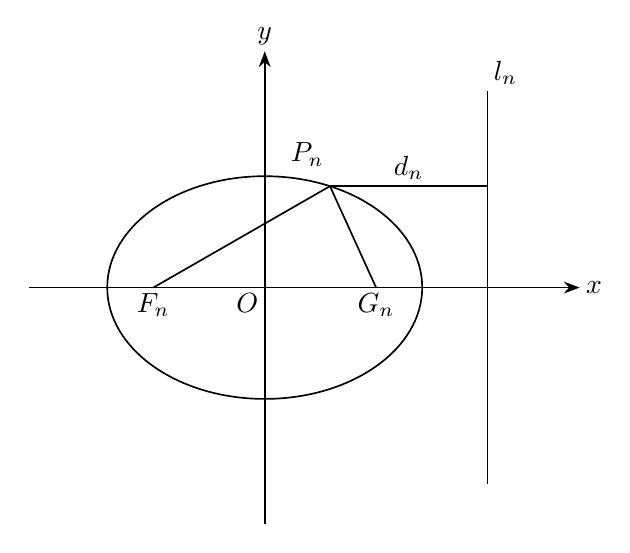
\begin{tikzpicture}[x=2cm,y=2cm,line width=.6pt,>=Stealth,font=\normalsize]
\coordinate (O) at (0.00000000,0.00000000);
\coordinate (Fn) at (-0.70710678,0.00000000);
\coordinate (Gn) at (0.70710678,0.00000000);
\coordinate (Pn) at (0.41421356,0.64359425);
\coordinate (Dn) at (1.41421356,0.64359425);
\coordinate (Lnbot) at (1.41421356,-1.25000000);
\coordinate (Lntop) at (1.41421356,1.25000000);
\coordinate (Xleft) at (-1.50000000,0.00000000);
\coordinate (Xright) at (2.00000000,0.00000000);
\coordinate (Ybot) at (0.00000000,-1.50000000);
\coordinate (Ytop) at (0.00000000,1.50000000);
\draw[->] (Xleft)--(Xright);
\draw[->] (Ybot)--(Ytop);
\draw (O) ellipse [x radius=1,y radius=0.70710678];
\draw (Lnbot)--(Lntop);
\draw (Pn)--(Fn);
\draw (Pn)--(Gn);
\draw (Pn)--(Dn);
\node[above left,inner sep=0pt,xshift=-2pt,yshift=7pt] at (Pn) {$P_n$};
\node[above,inner sep=0pt,yshift=2pt] at ($(Pn)!0.5!(Dn)$) {$d_n$};
\node[above right,inner sep=0pt,xshift=2pt,yshift=2pt] at (Lntop) {$l_n$};
\node[below,inner sep=0pt,yshift=-2pt] at (Fn) {$F_n$};
\node[below,inner sep=0pt,yshift=-2pt] at (Gn) {$G_n$};
\node[below left,inner sep=0pt,xshift=-2pt,yshift=-2pt] at (O) {$O$};
\node[right,inner sep=0pt,xshift=2pt] at (Xright) {$x$};
\node[above,inner sep=0pt,yshift=2pt] at (Ytop) {$y$};
\end{tikzpicture}
